\documentclass[12pt, fullpage,letterpaper]{article}

\usepackage[margin=1in]{geometry}
\usepackage{url}
\usepackage{amsmath}
\usepackage{amssymb}
\usepackage{xspace}
\usepackage{graphicx}
\usepackage{hyperref}
\usepackage{listings}

\newcommand{\semester}{Spring 2019}
\newcommand{\assignmentId}{1}
\newcommand{\releaseDate}{25 January, 2019}
\newcommand{\dueDate}{11:59pm, 10 Feb, 2019}

\newcommand{\bx}{{\bf x}}
\newcommand{\bw}{{\bf w}}

\title{CS 5350/6350: Machine Learining \semester}
\author{Homework \assignmentId}
\date{Handed out: \releaseDate\\
	Due: \dueDate}


\title{CS 5350/6350: Machine Learining \semester}
\author{Homework \assignmentId}
\date{Handed out: \releaseDate\\
  Due date: \dueDate}
  
%
% Various Helper Commands
%

% Alias for the Solution section header
\newcommand{\solution}{\textbf{\large Solution}}

\begin{document}
\maketitle

% Math commands by Thomas Minka
\newcommand{\var}{{\rm var}}
\newcommand{\Tr}{^{\rm T}}
\newcommand{\vtrans}[2]{{#1}^{(#2)}}
\newcommand{\kron}{\otimes}
\newcommand{\schur}[2]{({#1} | {#2})}
\newcommand{\schurdet}[2]{\left| ({#1} | {#2}) \right|}
\newcommand{\had}{\circ}
\newcommand{\diag}{{\rm diag}}
\newcommand{\invdiag}{\diag^{-1}}
\newcommand{\rank}{{\rm rank}}
% careful: ``null'' is already a latex command
\newcommand{\nullsp}{{\rm null}}
\newcommand{\tr}{{\rm tr}}
\renewcommand{\vec}{{\rm vec}}
\newcommand{\vech}{{\rm vech}}
\renewcommand{\det}[1]{\left| #1 \right|}
\newcommand{\pdet}[1]{\left| #1 \right|_{+}}
\newcommand{\pinv}[1]{#1^{+}}
\newcommand{\erf}{{\rm erf}}
\newcommand{\hypergeom}[2]{{}_{#1}F_{#2}}

% boldface characters
\renewcommand{\a}{{\bf a}}
\renewcommand{\b}{{\bf b}}
\renewcommand{\c}{{\bf c}}
\renewcommand{\d}{{\rm d}}  % for derivatives
\newcommand{\e}{{\bf e}}
\newcommand{\f}{{\bf f}}
\newcommand{\g}{{\bf g}}
\newcommand{\h}{{\bf h}}
%\newcommand{\k}{{\bf k}}
% in Latex2e this must be renewcommand
\renewcommand{\k}{{\bf k}}
\newcommand{\m}{{\bf m}}
\newcommand{\mb}{{\bf m}}
\newcommand{\n}{{\bf n}}
\renewcommand{\o}{{\bf o}}
\newcommand{\p}{{\bf p}}
\newcommand{\q}{{\bf q}}
\renewcommand{\r}{{\bf r}}
\newcommand{\s}{{\bf s}}
\renewcommand{\t}{{\bf t}}
\renewcommand{\u}{{\bf u}}
\renewcommand{\v}{{\bf v}}
\newcommand{\w}{{\bf w}}
\newcommand{\x}{{\bf x}}
\newcommand{\y}{{\bf y}}
\newcommand{\z}{{\bf z}}
%s\newcommand{\l}{\boldsymbol{l}}
\newcommand{\A}{{\bf A}}
\newcommand{\B}{{\bf B}}
\newcommand{\C}{{\bf C}}
\newcommand{\D}{{\bf D}}
\newcommand{\E}{{\bf E}}
\newcommand{\F}{{\bf F}}
\newcommand{\G}{{\bf G}}
\renewcommand{\H}{{\bf H}}
\newcommand{\I}{{\bf I}}
\newcommand{\J}{{\bf J}}
\newcommand{\K}{{\bf K}}
\renewcommand{\L}{{\bf L}}
\newcommand{\M}{{\bf M}}
\newcommand{\N}{\mathcal{N}}  % for normal density
%\newcommand{\N}{{\bf N}}
\renewcommand{\O}{{\bf O}}
\renewcommand{\P}{{\bf P}}
\newcommand{\Q}{{\bf Q}}
\newcommand{\R}{{\bf R}}
\renewcommand{\S}{{\bf S}}
\newcommand{\T}{{\bf T}}
\newcommand{\U}{{\bf U}}
\newcommand{\V}{{\bf V}}
\newcommand{\W}{{\bf W}}
\newcommand{\X}{{\bf X}}
\newcommand{\Y}{{\bf Y}}
\newcommand{\Z}{{\bf Z}}

% this is for latex 2.09
% unfortunately, the result is slanted - use Latex2e instead
%\newcommand{\bfLambda}{\mbox{\boldmath$\Lambda$}}
% this is for Latex2e
\newcommand{\bfLambda}{\boldsymbol{\Lambda}}

% Yuan Qi's boldsymbol
\newcommand{\bsigma}{\boldsymbol{\sigma}}
\newcommand{\balpha}{\boldsymbol{\alpha}}
\newcommand{\bpsi}{\boldsymbol{\psi}}
\newcommand{\bphi}{\boldsymbol{\phi}}
\newcommand{\boldeta}{\boldsymbol{\eta}}
\newcommand{\Beta}{\boldsymbol{\eta}}
\newcommand{\btau}{\boldsymbol{\tau}}
\newcommand{\bvarphi}{\boldsymbol{\varphi}}
\newcommand{\bzeta}{\boldsymbol{\zeta}}

\newcommand{\blambda}{\boldsymbol{\lambda}}
\newcommand{\bLambda}{\mathbf{\Lambda}}
\newcommand{\bOmega}{\mathbf{\Omega}}
\newcommand{\bomega}{\mathbf{\omega}}
\newcommand{\bPi}{\mathbf{\Pi}}

\newcommand{\btheta}{\boldsymbol{\theta}}
\newcommand{\bpi}{\boldsymbol{\pi}}
\newcommand{\bxi}{\boldsymbol{\xi}}
\newcommand{\bSigma}{\boldsymbol{\Sigma}}

\newcommand{\bgamma}{\boldsymbol{\gamma}}
\newcommand{\bGamma}{\mathbf{\Gamma}}

\newcommand{\bmu}{\boldsymbol{\mu}}
\newcommand{\1}{{\bf 1}}
\newcommand{\0}{{\bf 0}}

% \newcommand{\comment}[1]{}

\newcommand{\bs}{\backslash}
\newcommand{\ben}{\begin{enumerate}}
\newcommand{\een}{\end{enumerate}}

 \newcommand{\notS}{{\backslash S}}
 \newcommand{\nots}{{\backslash s}}
 \newcommand{\noti}{{\backslash i}}
 \newcommand{\notj}{{\backslash j}}
 \newcommand{\nott}{\backslash t}
 \newcommand{\notone}{{\backslash 1}}
 \newcommand{\nottp}{\backslash t+1}
% \newcommand{\notz}{\backslash z}

\newcommand{\notk}{{^{\backslash k}}}
%\newcommand{\noti}{{^{\backslash i}}}
\newcommand{\notij}{{^{\backslash i,j}}}
\newcommand{\notg}{{^{\backslash g}}}
\newcommand{\wnoti}{{_{\w}^{\backslash i}}}
\newcommand{\wnotg}{{_{\w}^{\backslash g}}}
\newcommand{\vnotij}{{_{\v}^{\backslash i,j}}}
\newcommand{\vnotg}{{_{\v}^{\backslash g}}}
\newcommand{\half}{\frac{1}{2}}
\newcommand{\msgb}{m_{t \leftarrow t+1}}
\newcommand{\msgf}{m_{t \rightarrow t+1}}
\newcommand{\msgfp}{m_{t-1 \rightarrow t}}

\newcommand{\proj}[1]{{\rm proj}\negmedspace\left[#1\right]}
\newcommand{\argmin}{\operatornamewithlimits{argmin}}
\newcommand{\argmax}{\operatornamewithlimits{argmax}}

\newcommand{\dif}{\mathrm{d}}
\newcommand{\abs}[1]{\lvert#1\rvert}
\newcommand{\norm}[1]{\lVert#1\rVert}

%miscellaneous symbols
\newcommand{\ie}{{{i.e.,}}\xspace}
\newcommand{\eg}{{{\em e.g.,}}\xspace}
\newcommand{\EE}{\mathbb{E}}
\newcommand{\VV}{\mathbb{V}}
\newcommand{\sbr}[1]{\left[#1\right]}
\newcommand{\rbr}[1]{\left(#1\right)}
\newcommand{\cmt}[1]{}


{\footnotesize
	Author: Cade Parkison
	
	Github: https://github.com/c-park/Machine-Learning-Library
	
}


\section{Decision Tree [40 points + 10 bonus]}

\begin{table}[h]
	\centering
	\begin{tabular}{cccc|c}
		$x_1$ & $x_2$ & $x_3$ & $x_4$ & $y$\\ 
		\hline\hline
		0 & 0 & 1 & 0 & 0 \\ \hline
		0 & 1 & 0 & 0 & 0 \\ \hline
		0 & 0 & 1 & 1 & 1 \\ \hline
		1 & 0 & 0 & 1 & 1 \\ \hline
		0 & 1 & 1 & 0.& 0\\ \hline
		1 & 1 & 0 & 0 & 0\\ \hline
		0 & 1 & 0 & 1 & 0\\ \hline
	\end{tabular}
	\caption{Training data for a Boolean classifier}
	%\caption{Training data for the alien invasion problem.}\label{tb-alien-train}
\end{table}

\begin{enumerate}
\item~[7 points] Decision tree construction. 



\begin{enumerate}
\item~

The following are the steps used in generating the decision tree using the ID3 algorithm:

	\begin{enumerate}
		\item Create a root node and calculate entropy of whole dataset
		\item For each of the four features $X_i$, calculate the information gain. Initially, both $X_2$ and $X_4$ give the same information gain, so I picked $x_2$ since it was first and assigned it to the root node. The info gain calculations are shown below.
		
		\[
        	\begin{split}
        		Gain(S,A) = Entropy(S) - \sum_v \frac{|S_v|}{|S|} Entropy(S_v)
        	\end{split}
		\]
		Where:
		\[
        	\begin{split}
        		Entropy(S) = \sum_{i=1}^k p_i \log_2 (p_i)
        	\end{split}
		\]
		
		\item For each feature value of $x_2$ (0 and 1), I added an unassigned branch to the tree.
		\item Then, I split the dataset on this $x_2$ feature and removed it from the dataset.
		\item Now there are two children of the root node, and each has it's own dataset. These subsets are shown below.
		
		\begin{table}[h]
			\centering
			\begin{tabular}{ccc|c}
				$x_1$  & $x_3$ & $x_4$ & $y$\\ 
				\hline\hline
				0 & 1 & 0 & 0 \\ \hline
				0 & 1 & 1 & 1 \\ \hline
				1 & 0 & 1 & 1 \\ \hline
	
			\end{tabular}
			\caption{$x_2=0$ data subset}
		
		\end{table}
		
		\begin{table}[h]
			\centering
			\begin{tabular}{ccc|c}
				$x_1$ & $x_3$ & $x_4$ & $y$\\ 
				\hline\hline

				0  & 0 & 0 & 0 \\ \hline
				0  & 1 & 0.& 0\\ \hline
				1  & 0 & 0 & 0\\ \hline
				0  & 0 & 1 & 0\\ \hline
	
			\end{tabular}
			\caption{$x_2=1$ data subset}
		
		\end{table}
		
		\item Repeating the steps above for the $x_2 = 0$ branch, I calculate entropy of this subset.
		\item I then calculate info gains for each remaining feature and split the subset on the one with the highest info gain, which is $x_4$.
		\item $x_4$ gets assigned to the $x_2 = 0$ branch, and the subset is split again into two branches, one for each feature value of $x_4$, these are shown below. 
		
		\begin{table}[h]
			\centering
			\begin{tabular}{cc|c}
				$x_1$ & $x_3$  & $y$\\ 
				\hline\hline

				0 & 1 & 0  \\ \hline

	
			\end{tabular}
			\caption{$x_2=0$ and $x_4=0$ data subset}
		
		\end{table}
		
		\begin{table}[h]
			\centering
			\begin{tabular}{cc|c}
				$x_1$ & $x_3$  & $y$\\ 
				\hline\hline
				
				0 & 1  & 1 \\ \hline
				1 & 0  & 1 \\ \hline
	
			\end{tabular}
			\caption{$x_2=0$ and $x_4=1$ data subset}
		
		\end{table}
		
		\item At the next level of recursion, I found that all target feature values are the same, so the $x_4$ branch of the tree ends. This can be seen in the above tables. 
		\item Returning to the $x_2 = 1$ branch, we see that the subset for this branch all have the same target feature value, meaning that if $x_2 = 1$ we can predict the outcome $y = 0$

	\end{enumerate}
	
	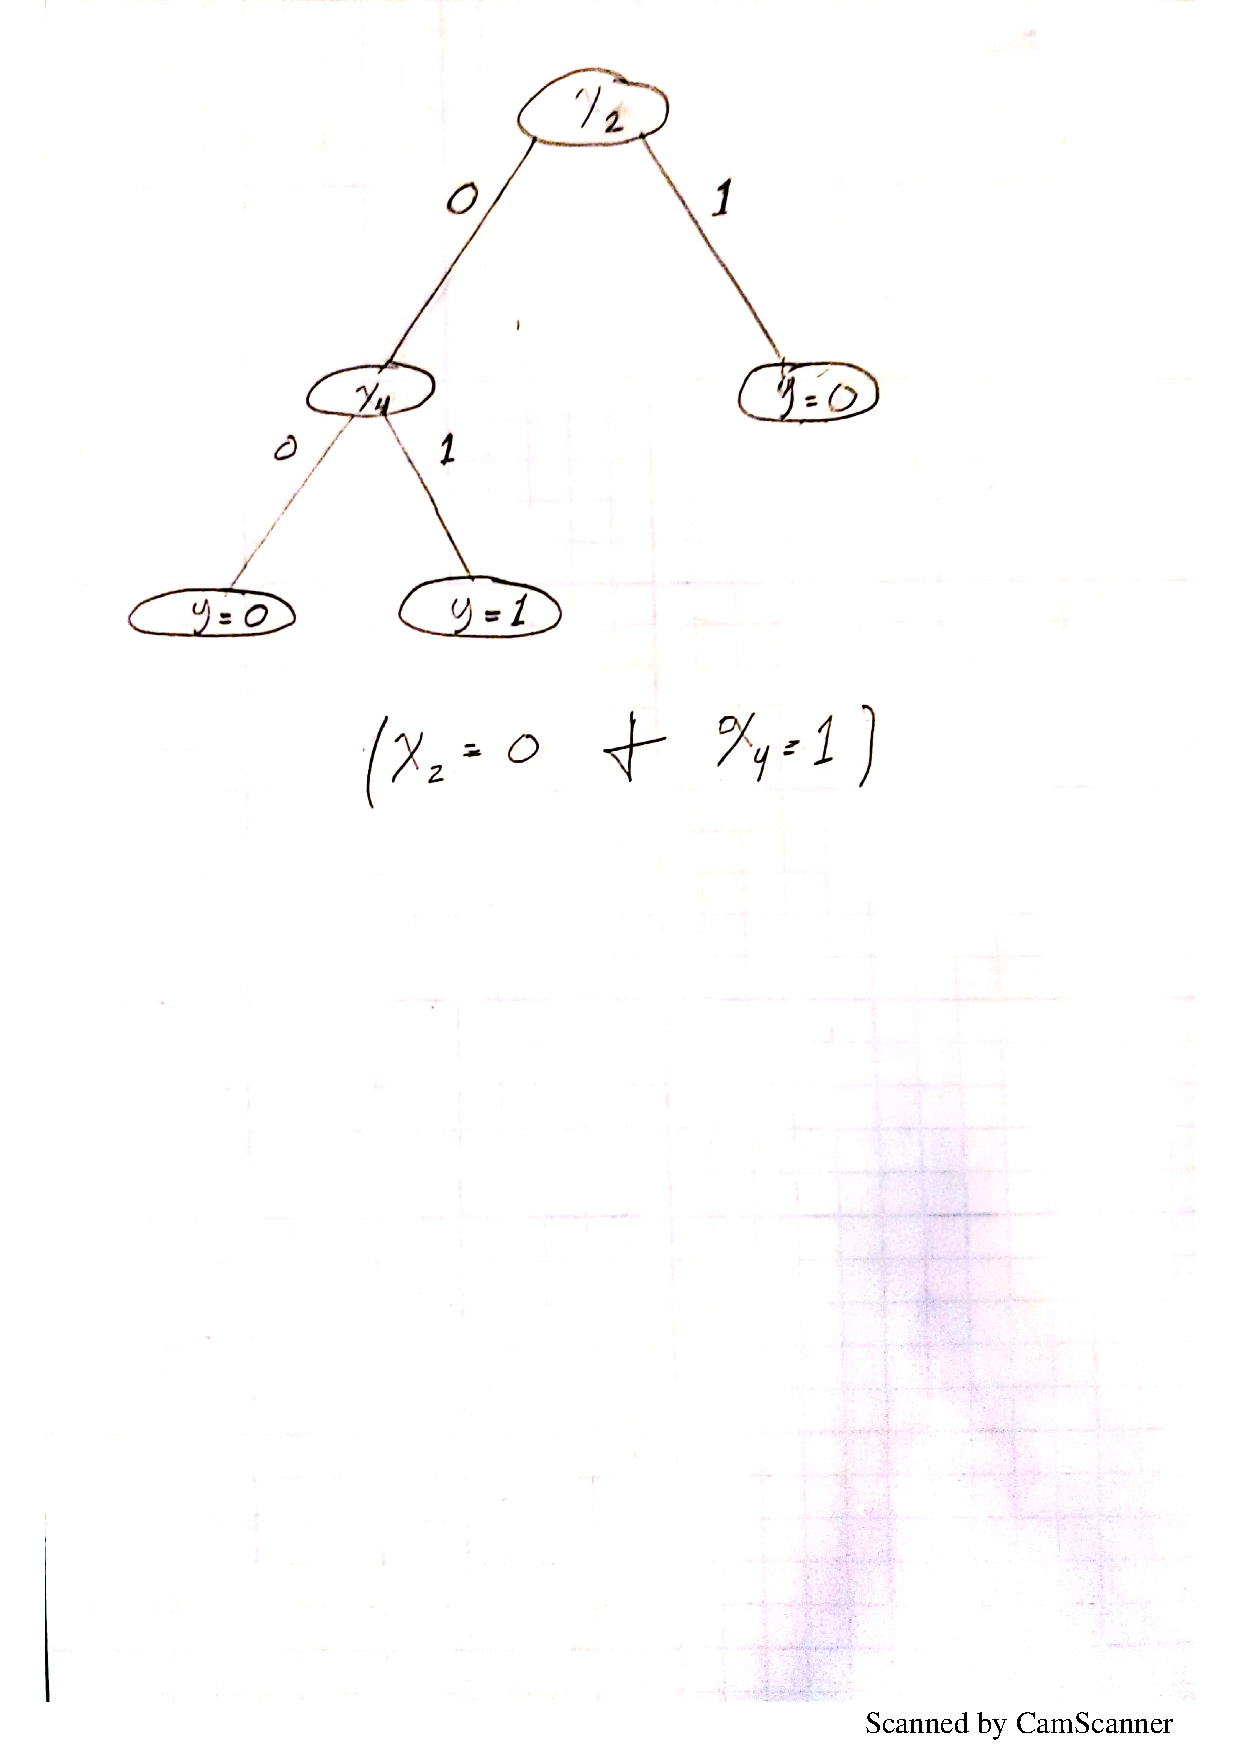
\includegraphics[]{tree1.pdf}

\item~ Boolean Representation:

	\[
        (x_2=0 \land x_4=1) 
	\]
	
	The above implicit equation is enough to fully describe the decision tree created in the previous problem.

\end{enumerate}


\item~
\label{sec:q2}
\begin{enumerate}
\item~

	Information gain using Majority Error:
	
	The following steps show the construction of the tree.
	
	\begin{enumerate}
		\item Create a root node and calculate majority error of whole dataset, $S$. Majority error is the error in labeling if the majority label were chosen. Since the majority of the examples are positive for playing tennis, this error is the ratio of negative examples to total examples.
		
			\[
        		ME(S) = \frac{5}{14}
			\]
		
		\item For each feature, calculate the information gain using majority error. The formula used and results are shown below.
		
			\[
        		\begin{split}
        			Gain(S,A) = ME(S) - \sum_v \frac{|S_v|}{|S|} ME(S_v)
        		\end{split}
			\]
			Info Gain for Outlook attribute (O):
			\[
        		\begin{split}
        			G(S,O) &= ME(S) - \sum_v \frac{|S_v|}{|S|} ME(S_v)
        					\\
        					&= ME(S) - \Big( \frac{|O=s|}{|S|} ME(O=s) +  \frac{|O=o|}{|S|} ME(O=o) + \frac{|O=r|}{|S|} ME(O=r)\Big)
        					\\
        					&= \frac{5}{14} - \Big( \frac{5}{14}\times\frac{2}{5} + \frac{4}{14}\times \frac{0}{4} + \frac{5}{14} \times \frac{2}{5}\Big)
        					\\
        					&= \frac{1}{14}
        		\end{split}
			\]
			
			Info Gain for Temperature attribute (T):
			\[
        		\begin{split}
        			G(S,T) &= \frac{5}{14} - \Big( \frac{4}{14}\times\frac{2}{4} + \frac{6}{14}\times \frac{2}{6} + \frac{4}{14} \times \frac{1}{4}\Big)
        					\\
        					&= 0
        		\end{split}
			\]
			
			Info Gain for Humidity attribute (H):
			\[
        		\begin{split}
        			G(S,H) &= \frac{5}{14} - \Big( \frac{7}{14}\times\frac{3}{7} + \frac{7}{14}\times \frac{1}{7} \Big)
        					\\
        					&= \frac{1}{14}
        		\end{split}
			\]
			
			Info Gain for Wind attribute (W):
			\[
        		\begin{split}
        			G(S,W) &= \frac{5}{14} - \Big( \frac{8}{14}\times\frac{2}{8} + \frac{6}{14}\times \frac{3}{6} \Big)
        					\\
        					&= 0
        		\end{split}
			\]
			
			Both the Outlook and Humidity attributes have the highest information gain, so either one of these can be chosen for the first node of our tree. I then chose the Outlook attribute to split the data. 
		\item For each attribute value of O, sunny overcast and rainy, I make a new branch of the tree. I then split the dataset based on this value, and remove the Overcast attribute from the data completely.
		
		\item I then repeat the above for each of the three data subsets by finding the best attribute to split the data subset based on the highest information gain.
		
		\item Starting with the Outlook=sunny data subset, shown below, we calculate the majority error.
		
		\begin{table}[h]
		\centering
		\begin{tabular}{ccc|c}
			T & H & W & Play?\\ 
			\hline\hline
			H & H & W & -\\ \hline
			H & H & S & -\\ \hline
			M & H & W & -\\ \hline
			C & N & W & +\\ \hline
			M & N & S & +\\ \hline

		\end{tabular}
		\caption{Outlook=sunny data subset}
		%\caption{Training data for the alien invasion problem.}\label{tb-alien-train}
		\end{table}		
		
		\[
			ME(S_{O=sunny}) = \frac{2}{5}
		\]
		
		\item Next, I calculate the info gain for each of the remaining attributes using the same formulas as above.
		
		\[
			Gain(T) = 0.32
		\]
		\[
			Gain(H) = 0.4
		\]
		\[
			Gain(W) = 0
		\]
		
		\item As can be seen, the Humidity attribute has the highest information gain, so we split the subset on these attribute values and create new tree branches with them. 
		
		\item For the O=sunny and Humidity data subset, all remaining subsets have equal target values. O=sunny and H=high gives Play=-, while O=sunny and H=low gives Play=+. We now traverse back up the tree and continue the recursion. 
		
		\item All O=overcast data have the target value of Play=+, so this branch is also complete.
		
		\item Finally, we take the O=rainy data subset and find the info gains for each remaining attribute. In this case, the Wind attribute gives the highest gain, so we split the remaining data on these attribute values.
		
		\item After splitting again, we see all remaining data have the same target values, so the tree is complete. See the picture below.
		
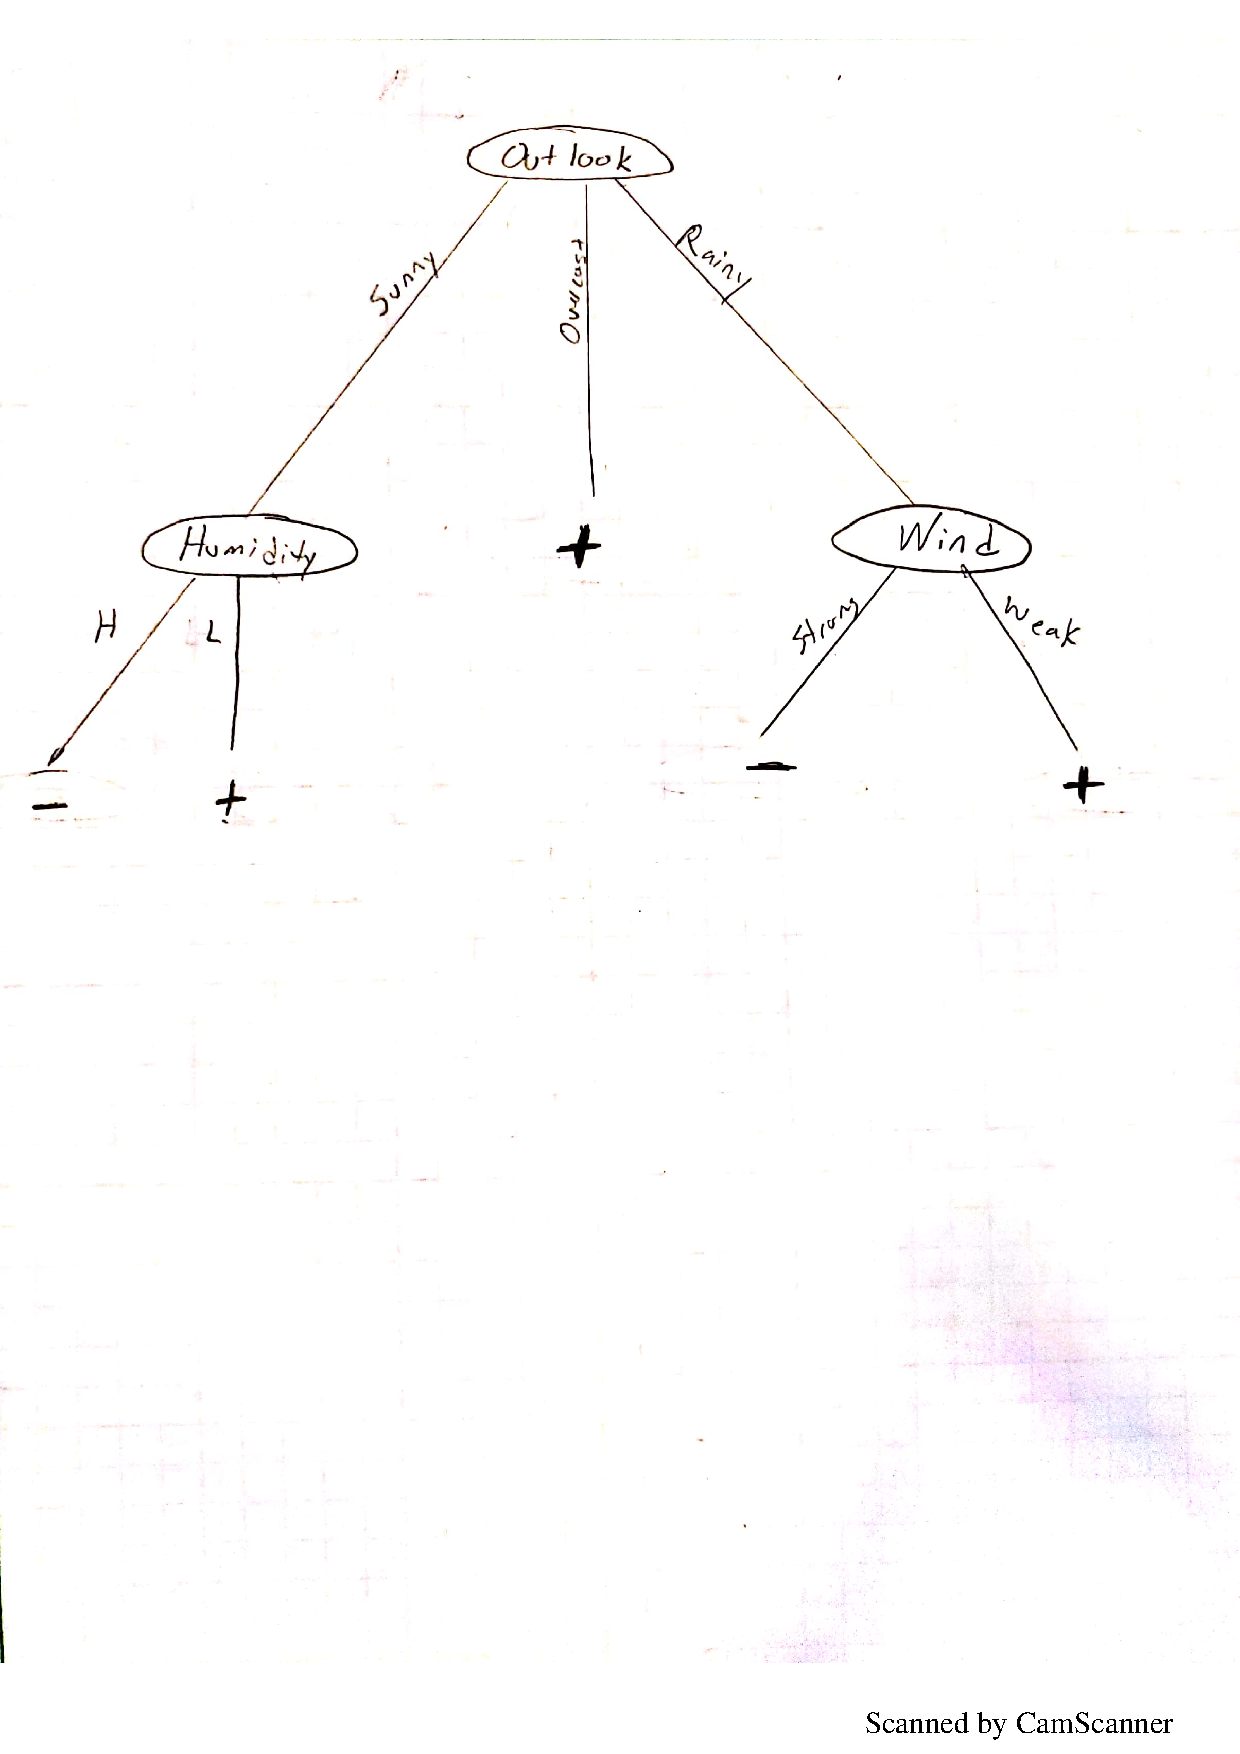
\includegraphics[]{tree_me.pdf}
			
	\end{enumerate}
	
	

\item~

	Gini Index:
	
	The following steps are used to construct a tree using the Gini index.
	
	\begin{enumerate}
		\item Create root node and calculate Gini index of complete data set. 
		
		\[
			\begin{split}
				GI(S) &= 1 - ( p_{-}^2 + p_{+}^2)
					\\
					&= 1 - (\frac{9}{14})^2 - (\frac{5}{14})^2
					\\
					&= \frac{45}{98}
					\\
					&= 0.45918
			\end{split}
		\]
		
		\item For each feature, calculate information gain using this Gini index.
		
		\[
			\begin{split}
				Gain(S,A) &= GI(S) - \sum_v \frac{|S_v|}{|S|} GI(S_v)
					\\
					&=
					\\
					&= 
					\\
					&=
			\end{split}
		\]
		
		Info Gain for Outlook attribute (O):
		\[
        		\begin{split}
        			G(S,O) &= GI(S) - \sum_v \frac{|S_v|}{|S|} GI(S_v)
        					\\
        					&= \frac{45}{98} - \Big( \frac{5}{14}\times (1 - (\frac{2}{5})^2 - (\frac{3}{5})^2) + \frac{4}{14}\times (1 - (\frac{4}{4})^2 - (\frac{0}{4})^2) + \frac{5}{14} \times (1 - (\frac{3}{5})^2 - (\frac{2}{5})^2)\Big)
        					\\
        					&= \frac{45}{98} - \Big( \frac{5}{14}\times (\frac{12}{25}) + \frac{4}{14}\times (0) + \frac{5}{14} \times (\frac{12}{25})\Big)
        					\\
        					&= 0.1163
        		\end{split}
			\]
			
		Info Gain for Temperature attribute (T):
		\[
        		\begin{split}
        			G(S,T) &= GI(S) - \sum_v \frac{|S_v|}{|S|} GI(S_v)
        					\\
        					&= \frac{45}{98} - \Big( \frac{4}{14}\times (1 - (\frac{2}{4})^2 - (\frac{2}{4})^2) + \frac{6}{14}\times (1 - (\frac{4}{6})^2 - (\frac{2}{6})^2) + \frac{4}{14} \times (1 - (\frac{3}{4})^2 - (\frac{1}{4})^2)\Big)
        					\\
        					&= \frac{45}{98} - \Big( \frac{4}{14}\times (\frac{1}{2}) + \frac{6}{14}\times (\frac{4}{9}) + \frac{4}{14} \times (\frac{3}{8})\Big)
        					\\
        					&= 0.0197
        		\end{split}
			\]
			
		Info Gain for Humidity attribute (H):
		\[
        		\begin{split}
        			G(S,H) &= GI(S) - \sum_v \frac{|S_v|}{|S|} GI(S_v)
        					\\
        					&= \frac{45}{98} - \Big( \frac{7}{14}\times (1 - (\frac{3}{7})^2 - (\frac{4}{7})^2) + \frac{7}{14}\times (1 - (\frac{6}{7})^2 - (\frac{1}{7})^2) \Big)
        					\\
        					&= \frac{45}{98} - \Big( \frac{7}{14}\times (\frac{24}{49}) + \frac{7}{14}\times (\frac{12}{49}) \Big)
        					\\
        					&= 0.0918
        		\end{split}
			\]
			
		Info Gain for Wind attribute (W):
		\[
        		\begin{split}
        			G(S,W) &= GI(S) - \sum_v \frac{|S_v|}{|S|} GI(S_v)
        					\\
        					&= \frac{45}{98} - \Big( \frac{8}{14}\times (1 - (\frac{6}{8})^2 - (\frac{2}{8})^2) + \frac{6}{14}\times (1 - (\frac{3}{6})^2 - (\frac{3}{6})^2) \Big)
        					\\
        					&= \frac{45}{98} - \Big( \frac{8}{14}\times (\frac{3}{8}) + \frac{6}{14}\times (\frac{1}{2}) \Big)
        					\\
        					&= 0.0306
        		\end{split}
			\]
			
		\item Since Outlook has the highest information gain, we choose this as our root node and split the dataset according to Outlook values. 
		
				\item For each attribute value of O, sunny overcast and rainy, I make a new branch of the tree. I then split the dataset based on this value, and remove the Overcast attribute from the data completely.
		
		\item I then repeat the above for each of the three data subsets by finding the best attribute to split the data subset based on the highest information gain.
		
		\item I now will repeat the above steps for the Outlook=sunny data subset. The gini index for this subset is the following.
		
		\[
			GI = 1 - (\frac{3}{5})^2 - (\frac{2}{5})^2 = \frac{12}{25}
		\]
		
		\item Next, I calculate the info gain for the remaining three attributes. These values are shown below.
		
		\[
			Gain(T) = 0.28
		\]
		\[
			Gain(H) = 0.48
		\]
		\[
			Gain(W) = 0.0133
		\]
		
		Since the Humidity attribute has the highest info gain, I choose this as the attribute to split the remaining data on. After the split, the data subsets all have the same target values, so we move back up the tree.
		
		
		
	\end{enumerate}

\item~ Comparing the two trees I just created to the one in the lecture notes, all the trees look the same. There are no differences due to the way the data is arranged. The individual information gains are different for each of the three cases, but the ratios between each attribute remain fairly similar. This has the effect of choosing the same attributes for splitting regardless of the information gain method.

\end{enumerate}

\pagebreak


\item~
\begin{enumerate}
\item~

		For the attribute Outlook, the most common value is both S and R, so I picked S as the missing value. Using the original information gain with entropy, I calculate the entropy of the entire new data set first.
		
		\[
			\begin{split}
				H &= -\frac{10}{15} \log_2 (\frac{10}{15}) - \frac{5}{15} \log_2 (\frac{5}{15})
					\\
					&= 0.9183			
			\end{split}
		\]
		
		Information gain for Outlook attribute:
		
		
		\[
			\begin{split}
				IG &= H - [\frac{6}{15}H_{O=s} + \frac{4}{15} H_{O=o} + \frac{5}{15} H_{O=r}]
					\\
					&= 0.9183	 - [\frac{6}{15}(1) + \frac{4}{15}(0) + \frac{5}{15} (0.97)]	
					\\
					&= 	0.1943
			\end{split}
		\]
		
		Information gain for Temperature attribute:
		
		
		\[
			\begin{split}
				IG &= H - [\frac{4}{15}H_{t=hot} + \frac{7}{15} H_{t=m} + \frac{4}{15} H_{t=c}]
					\\
					&= 0.9183	 - [\frac{4}{15}(1) + \frac{7}{15}(0.985) + \frac{4}{15} (0.97)]	
					\\
					&= 	-0.06
			\end{split}
		\]
		
		Information gain for Humidity attribute:
		
		
		\[
			\begin{split}
				IG &= H - [\frac{7}{15}H_{h=h} + \frac{8}{15} H_{h=n}]
					\\
					&= 0.9183	 - [\frac{7}{15}(0.985) + \frac{8}{15}(0.543)]	
					\\
					&= 	0.169
			\end{split}
		\]
		
		Information gain for Wind attribute:
		
		
		\[
			\begin{split}
				IG &= H - [\frac{9}{15}H_{w=w} + \frac{6}{15} H_{w=s}]
					\\
					&= 0.9183	 - [\frac{9}{15}(0.764) + \frac{6}{15}(1)]	
					\\
					&= 	0.0599
			\end{split}
		\]
		
		As can be seen above, the best feature (highest gain) is the Outlook feature. 



\end{enumerate}

\item ~[\textbf{Bonus question 1}]

\item ~[\textbf{Bonus question 2}]

\end{enumerate}

\pagebreak


\section{Decision Tree Practice [60 points]}
\begin{enumerate}
	\item~[5 Points] 


\item~



\begin{enumerate}
\item~

\item~ 
	After implementing my algorithm, I learned decision trees from the training data and tested them against the test data. I varied the tree depth from 1 to 6 as well. The percent errors for both data sets are shown below for entropy, majority error, and gini index.

		\begin{table}[h]
		\centering
		\begin{tabular}{c|cc}
			Max Depth & Training & Testing\\ 
			\hline\hline
			1 & 30.20 & 29.67  \\ \hline
			2 & 22.19 & 22.25  \\ \hline
			3 & 18.10 & 19.64  \\ \hline
			4 & 8.19 & 15.11  \\ \hline
			5 & 2.70 & 9.89 \\ \hline
			6 & 0.0 & 12.22  \\ \hline

		\end{tabular}
		\caption{Percent errors with entropy}
		
		\end{table}	
		
		\begin{table}[h]
		\centering
		\begin{tabular}{c|cc}
			Max Depth & Training & Testing\\ 
			\hline\hline
			1 & 30.20 & 29.67  \\ \hline
			2 & 29.20 & 31.32  \\ \hline
			3 & 19.29 & 21.15  \\ \hline
			4 & 11.09 & 17.86  \\ \hline
			5 & 3.6 & 12.36 \\ \hline
			6 & 0.0 & 14.84  \\ \hline

		\end{tabular}
		\caption{Percent errors with majority error}
		
		\end{table}	
		
		\begin{table}[h]
		\centering
		\begin{tabular}{c|cc}
			Max Depth & Training & Testing\\ 
			\hline\hline
			1 & 30.20 & 29.67  \\ \hline
			2 & 22.19 & 22.25  \\ \hline
			3 & 17.6 & 18.41  \\ \hline
			4 & 8.90 & 13.74  \\ \hline
			5 & 2.70 & 9.89 \\ \hline
			6 & 0.0 & 12.22  \\ \hline

		\end{tabular}
		\caption{Percent errors with gini index}
		
		\end{table}	

\item~

	As can be seen in the above tables, the overall accuracy of my algorithm is fairly high, especially at high max depth numbers. In all three cases, the worst error seen at a depth of 6 is less than 15\%. Comparing the three types of information gain, we can see that the gini index gave the best results, but not by much. Both gini index and info gain results are very similar, with only slight differences at certain max depths. Majority error showed promising results as well, only slightly worse than the other two. Comparing the training and testing errors, we can see both have similar errors at low max depth. As the depth increases, the training errors converge to zero, while the testing errors converge to an error around 12\%. This makes sense, as the tree will overfit the training data if it can. Another interesting point is that the lowest testing errors were at a max depth of 5, which also confirms the overfitting issue. 
	

\end{enumerate}


\item~[25 points] 
\begin{enumerate}
	\item~ Unknown as a particular attribute value
	
		\begin{table}[h]
		\centering
		\begin{tabular}{c|cc}
			Max Depth & Training & Testing\\ 
			\hline\hline
			1 & 11.92 & 12.48  \\ \hline
			2 & 10.60 & 11.14  \\ \hline
			3 & 10.06 & 10.70  \\ \hline
			4 & 7.92 & 11.50  \\ \hline
			5 & 6.12 & 12.2 \\ \hline
			6 & 4.72 & 13.24  \\ \hline
			7 & 3.48 & 14.22  \\ \hline
			8 & 2.86 & 14.64 \\ \hline
			9 & 2.30 & 15.08  \\ \hline
			10 & 1.70 & 15.54  \\ \hline
			11 & 1.44 & 15.62  \\ \hline
			12 & 1.36 & 15.56  \\ \hline
			13 & 1.36 & 15.56  \\ \hline
			14 & 1.36 & 15.54  \\ \hline
			15 & 1.36 & 15.54  \\ \hline
			16 & 1.36 & 15.54  \\ \hline

		\end{tabular}
		\caption{Percent errors with entropy}
		
		\end{table}
		
		\begin{table}[h]
		\centering
		\begin{tabular}{c|cc}
			Max Depth & Training & Testing\\ 
			\hline\hline
			1 & 10.88 & 11.66  \\ \hline
			2 & 10.42 & 10.88  \\ \hline
			3 & 9.60 & 11.21  \\ \hline
			4 & 8.18 & 11.82  \\ \hline
			5 & 7.18 & 11.68 \\ \hline
			6 & 6.74 & 11.94  \\ \hline
			7 & 6.44 & 12.04  \\ \hline
			8 & 5.92 & 12.32 \\ \hline
			9 & 5.08 & 12.84  \\ \hline
			10 & 4.28 & 13.8  \\ \hline
			11 & 3.84 & 14.2  \\ \hline
			12 & 3.24 & 14.74  \\ \hline
			13 & 2.76 & 15.1  \\ \hline
			14 & 2.02 & 15.58  \\ \hline
			15 & 1.54 & 15.76  \\ \hline
			16 & 1.36 & 15.76  \\ \hline

		\end{tabular}
		\caption{Percent errors with majority error}
		
		\end{table}
	
	\item~ Unknown as attribute value missing
	
	
	\item~ As can be seen in the above tables, there is an optimal tree depth where the testing data performs the best. This depth is lower than the max depth, and appeared to be around a depth of two or three for the results above. This is due to the model overfitting the training data. 
\end{enumerate}
\end{enumerate}




\end{document}
%%% Local Variables:
%%% mode: latex
%%% TeX-master: t
%%% End:
